\chapter{Implementation}
\graphicspath{{Chapter4/Figs/}{Chapter4/Figs/}}

This chapter goes into the implementation details of building the software parts for the NIP of IDUN and the key events that occurred during the empirical software engineering process, such as the realisation of the novelty and the need for a definition for a N/CI. Next to that, the author also discusses other key aspects and learnings from building the system.

\section{Timeline}
\label{chapter4-timeline}

Procedures, such as enlisted in the project stages presented in \autoref{chapter3-project-stages}, are a good guide for project implementation, but in the end, such plans run in unexpected ways. As a result, researching and implementing a non-trivial system such as a N/CI requires a high level of agility.

The effective timeline at the time of writing is shown in \autoref{fig:implementation-timeline}. It includes the previously mentioned project stages but is differently structured as initially described. \autoref{tab:special-project-stages} explains why some project stages were completed differently than initially planned.

\begin{figure}[!ht]
  \centering
  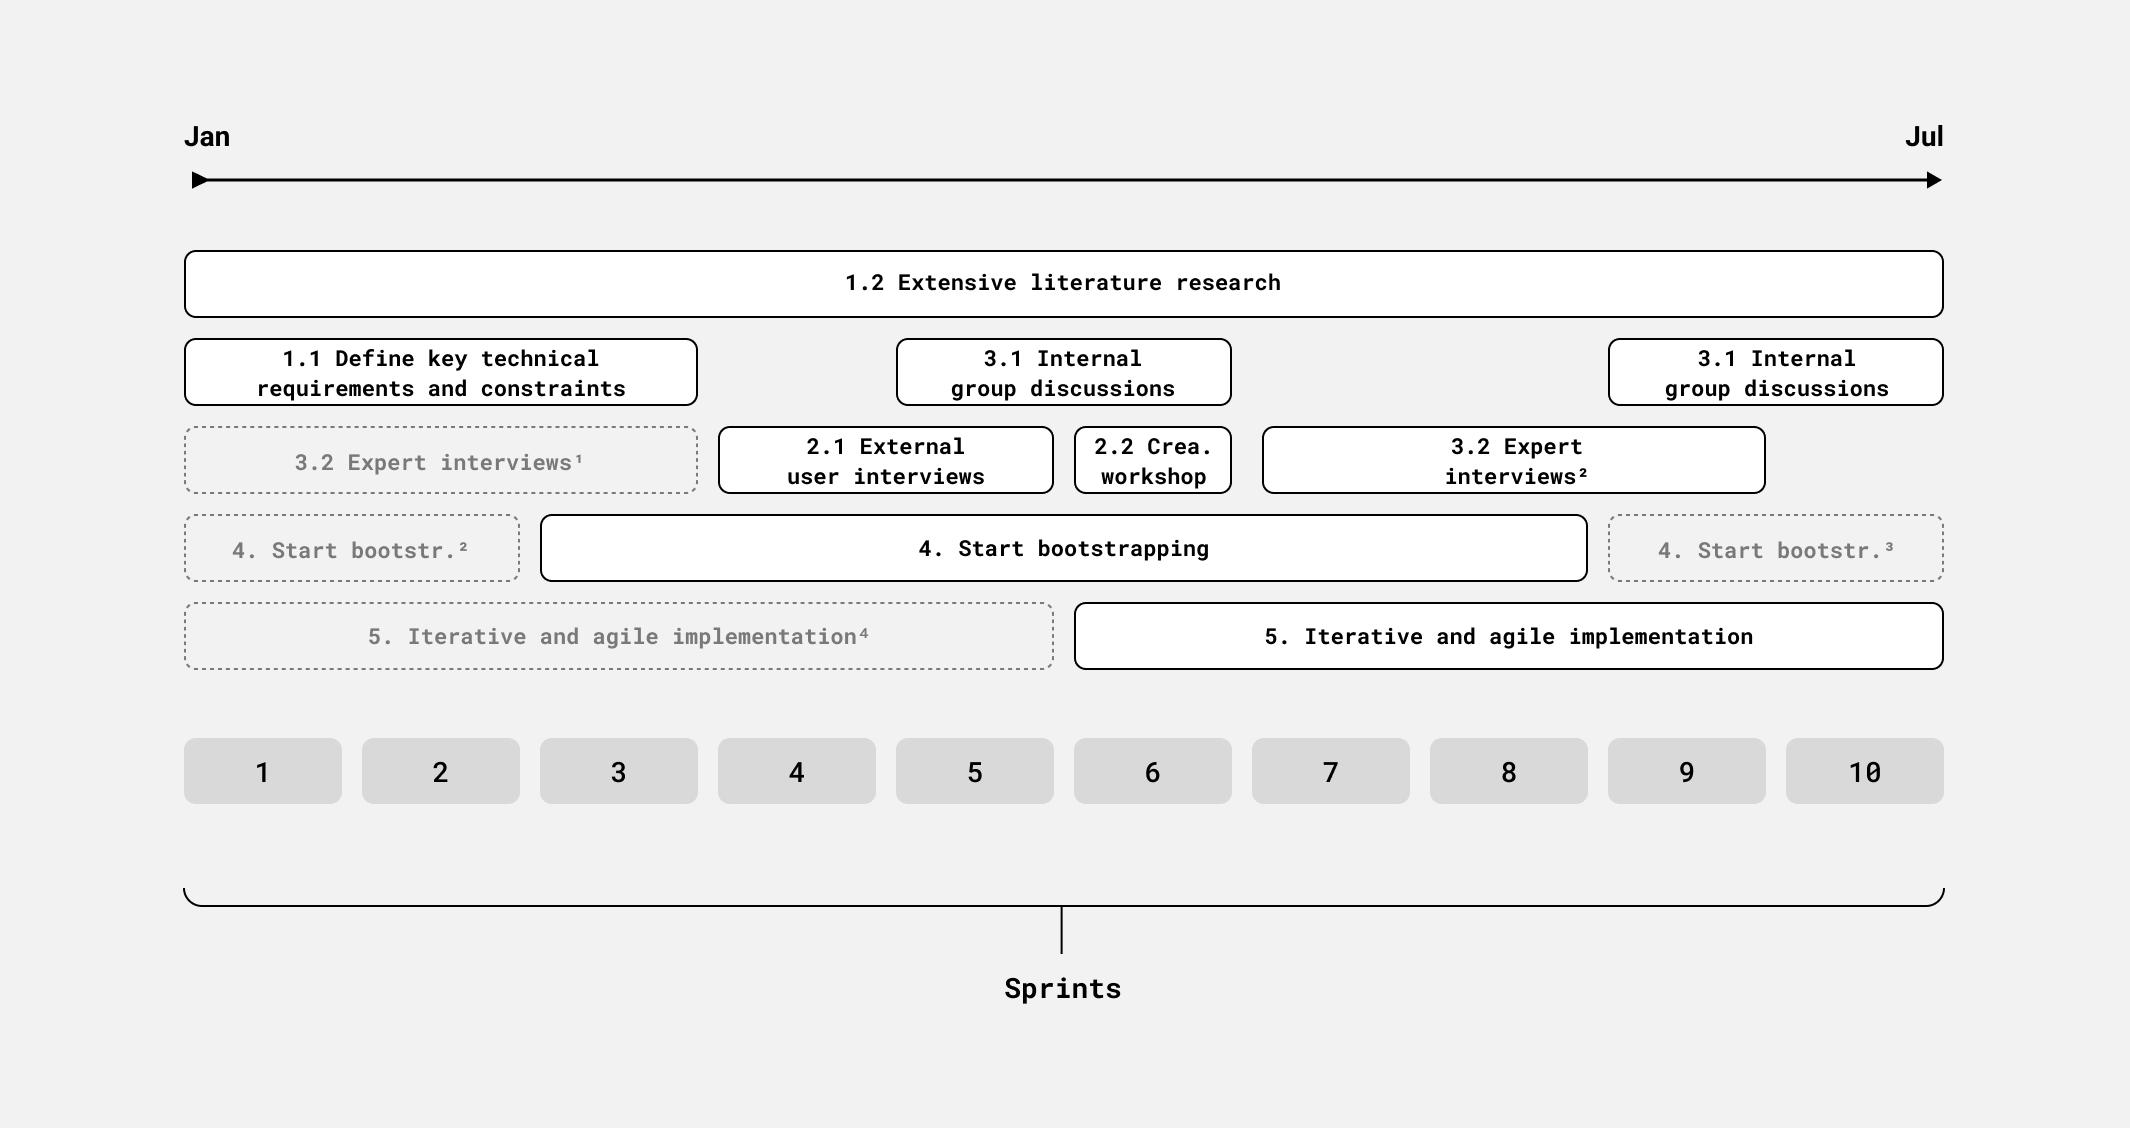
\includegraphics[width=\linewidth]{implementation-timeline.png}
  \caption{Effective timeline of the last ten sprints with project stages in white and specifically planned stages outlined in grey.}
  \label{fig:implementation-timeline}
\end{figure}

\begin{table}[ht]
\centering
\resizebox{\textwidth}{!}{%
\begin{tabular}{
>{\columncolor[HTML]{FFFFFF}}l l}
\cellcolor[HTML]{000000}{\color[HTML]{FFFFFF} Special stage} &
  \cellcolor[HTML]{000000}{\color[HTML]{FFFFFF} Description} \\ \hline
\multicolumn{1}{|l|}{\cellcolor[HTML]{FFFFFF}\textbf{\begin{tabular}[c]{@{}l@{}}[1] 3.2 Expert\\ interviews\end{tabular}}} &
  \multicolumn{1}{l|}{\begin{tabular}[c]{@{}l@{}}The author was able to use the first expert discussions in advance thanks to the help of one\\ of the sales staff's networks. The experts were Nuvibit's experienced enterprise cloud and\\ solution architects. The first topics were strictly technical in nature, focusing on medium-\\ term technological decisions in the context of the company and the timetable.\end{tabular}} \\ \hline
\multicolumn{1}{|l|}{\cellcolor[HTML]{FFFFFF}\textbf{\begin{tabular}[c]{@{}l@{}}[2] 4. Start\\ bootstrapping\end{tabular}}} &
  \multicolumn{1}{l|}{\begin{tabular}[c]{@{}l@{}}This special stage describes the phase in which the author established more organisational\\ structures, such as a professional Scrum or GitHub setup. Furthermore, the time was used\\ to create a more professional AWS organisational setup with various organisational units,\\ as described in the AWS Best Practice Guide \citep{blackham_best_2020}.\end{tabular}} \\ \hline
\multicolumn{1}{|l|}{\cellcolor[HTML]{FFFFFF}\textbf{\begin{tabular}[c]{@{}l@{}}[3] 4. Start\\ bootstrapping\end{tabular}}} &
  \multicolumn{1}{l|}{\begin{tabular}[c]{@{}l@{}}Since the creation of two different Python SDKs (as discussed later in the thesis), more\\ bootstrapping tasks were due at the very end of the given time frame, mostly including\\ the setup of a private PyPi installable Python package and SDK-specific quality\\ assurance pipelines and automations.\end{tabular}} \\ \hline
\multicolumn{1}{|l|}{\cellcolor[HTML]{FFFFFF}\textbf{\begin{tabular}[c]{@{}l@{}}[4] 5. Iterative and\\ agile implementation\end{tabular}}} &
  \multicolumn{1}{l|}{\begin{tabular}[c]{@{}l@{}}Iterative and agile implementation began as soon as needed, without waiting for the design\\ process to be completed (i.e. avoiding a waterfall process). Prior to gaining insights from the \\ design process, time was spent on everything else, such as evaluating technologies, further\\ bootstrapping, first example codebases, or maintaining the old codebase a bit.\end{tabular}} \\ \hline
\end{tabular}%
}
\vspace{10pt}
\caption{Special project stages in the effective schedule as shown in \autoref{fig:implementation-timeline} and their explanation of why they took place there.}
\vspace{-5pt}
\label{tab:special-project-stages}
\end{table}

Several key events occurred during the implementation that shaped the future course of the project and research. This was primarily due to early expert discussions or uncertainties in the requirements as the user-centred design process was still being prepared. These key events are overlaid with the effective project plan as shown in \autoref{fig:implementation-timeline-key-events}. These three green key events are the most influential key events.

\begin{figure}[!ht]
  \centering
  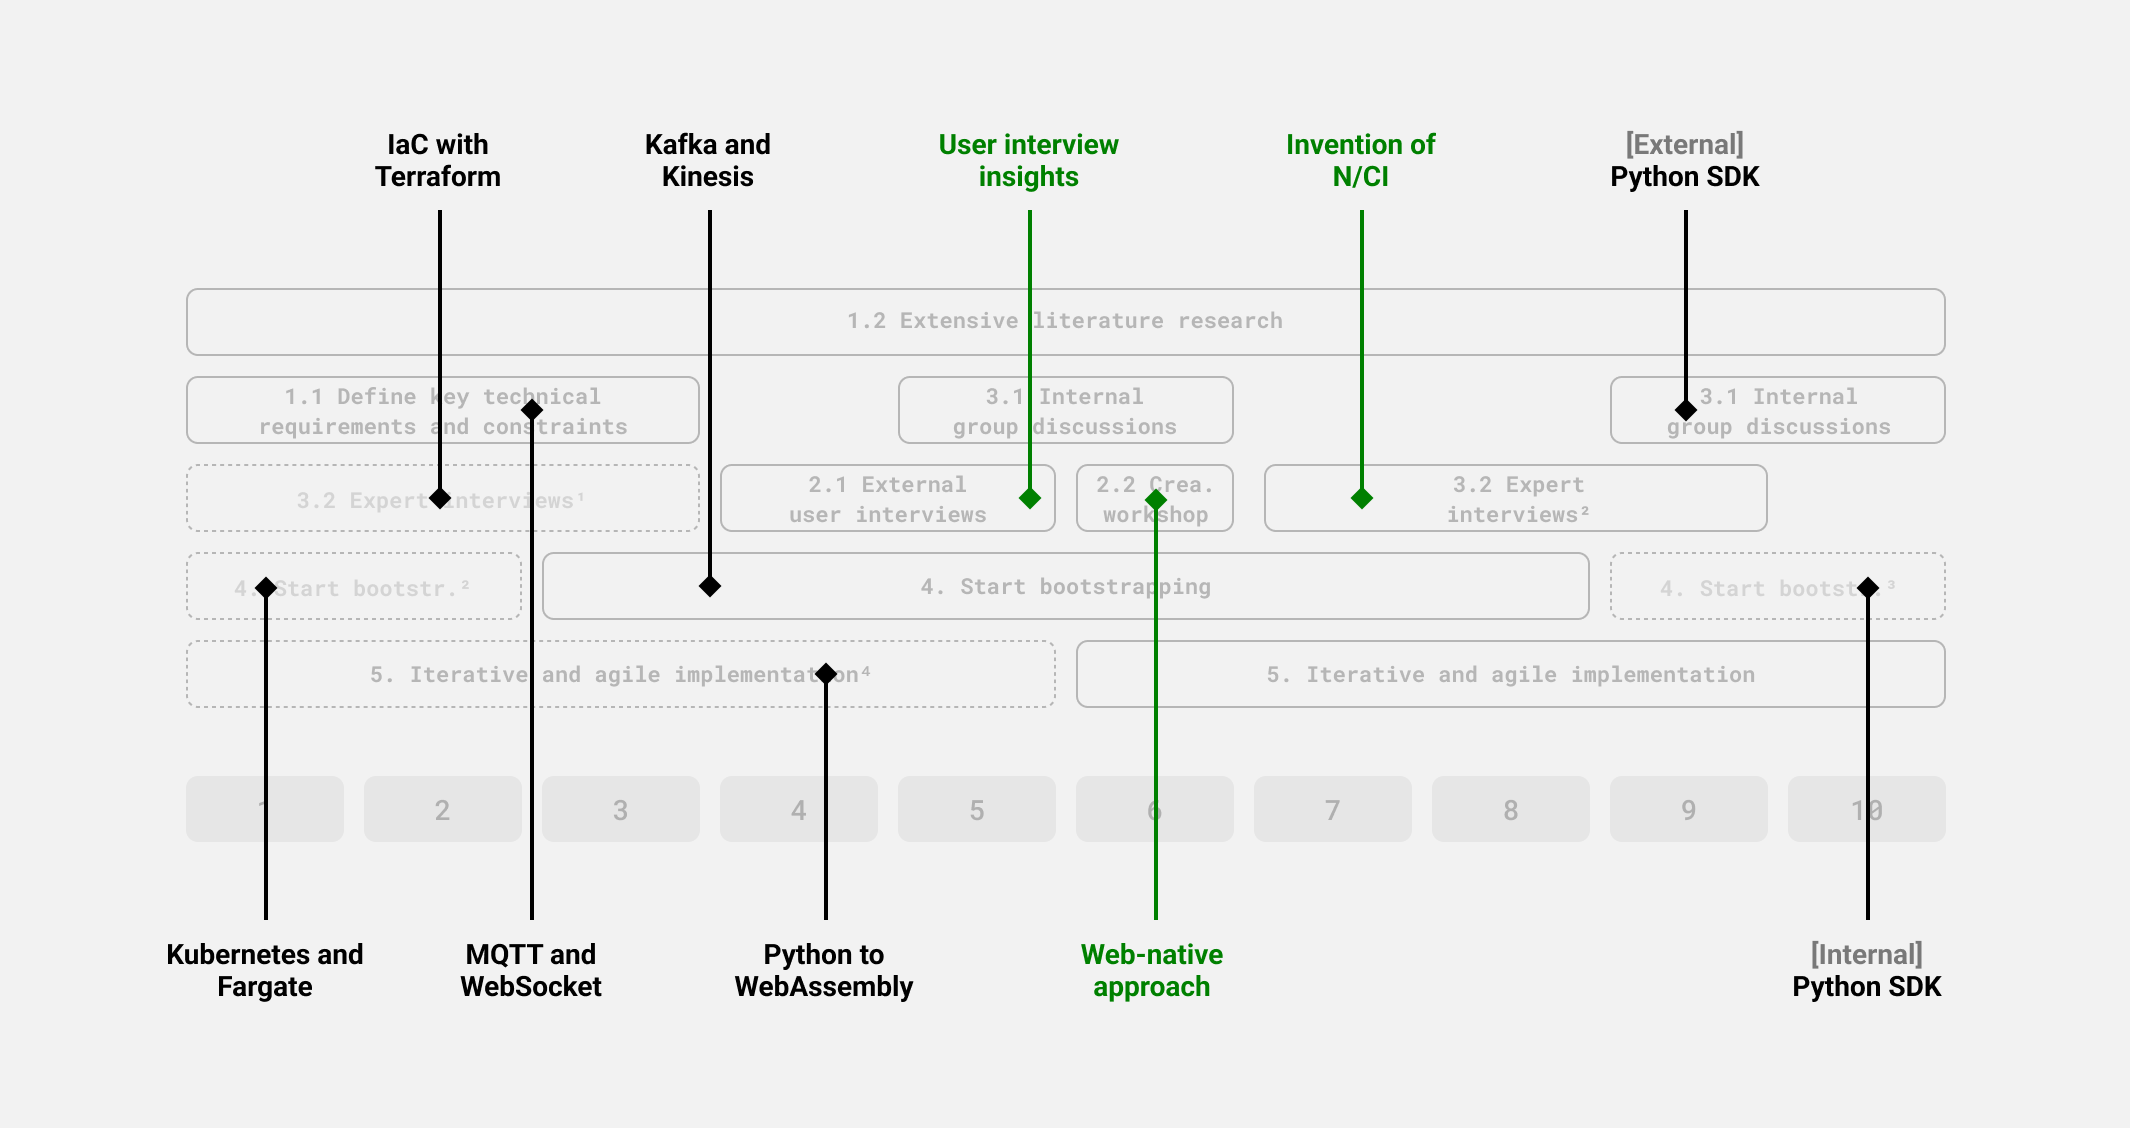
\includegraphics[width=\linewidth]{implementation-timeline-key-events.png}
  \caption{The key events overlaid on the effective project schedule as illustrated in \autoref{fig:implementation-timeline}, with the most influential events coloured green.}
  \label{fig:implementation-timeline-key-events}
\end{figure}

% empirical software engineering done in the case study based on a user-centred design process via user interviews, expert interviews, internal group discussions, and ongoing literature research.
% MENTION analysis paralysis

\section{Key events}
\label{chapter4-key-events}

This section goes over each key event as shown in \autoref{fig:implementation-timeline-key-events} and discusses why it happened and was critical to the project's success. The following outline of the key events is not chronologically described but instead starts with the most influential ones, which were previously coloured green.

\subsection{User interview insights}
\label{chapter4-user-interview-insights}

The conduct of user interviews was one of the most influential key events. This process began with the development of customer personas based on the sales team's previous experiences with real customers and the planned customer segments targeted by C-level management. The author does not want to go into too much detail about how the personas were created and how the process went, because the focus is on the results based on the personas, not on the persona creation process itself. The personas are illustrated in \autoref{fig:personas}, and a more detailed version is included in \autoref{appendix4-screenshots}.

\begin{figure}[!ht]
  \centering
  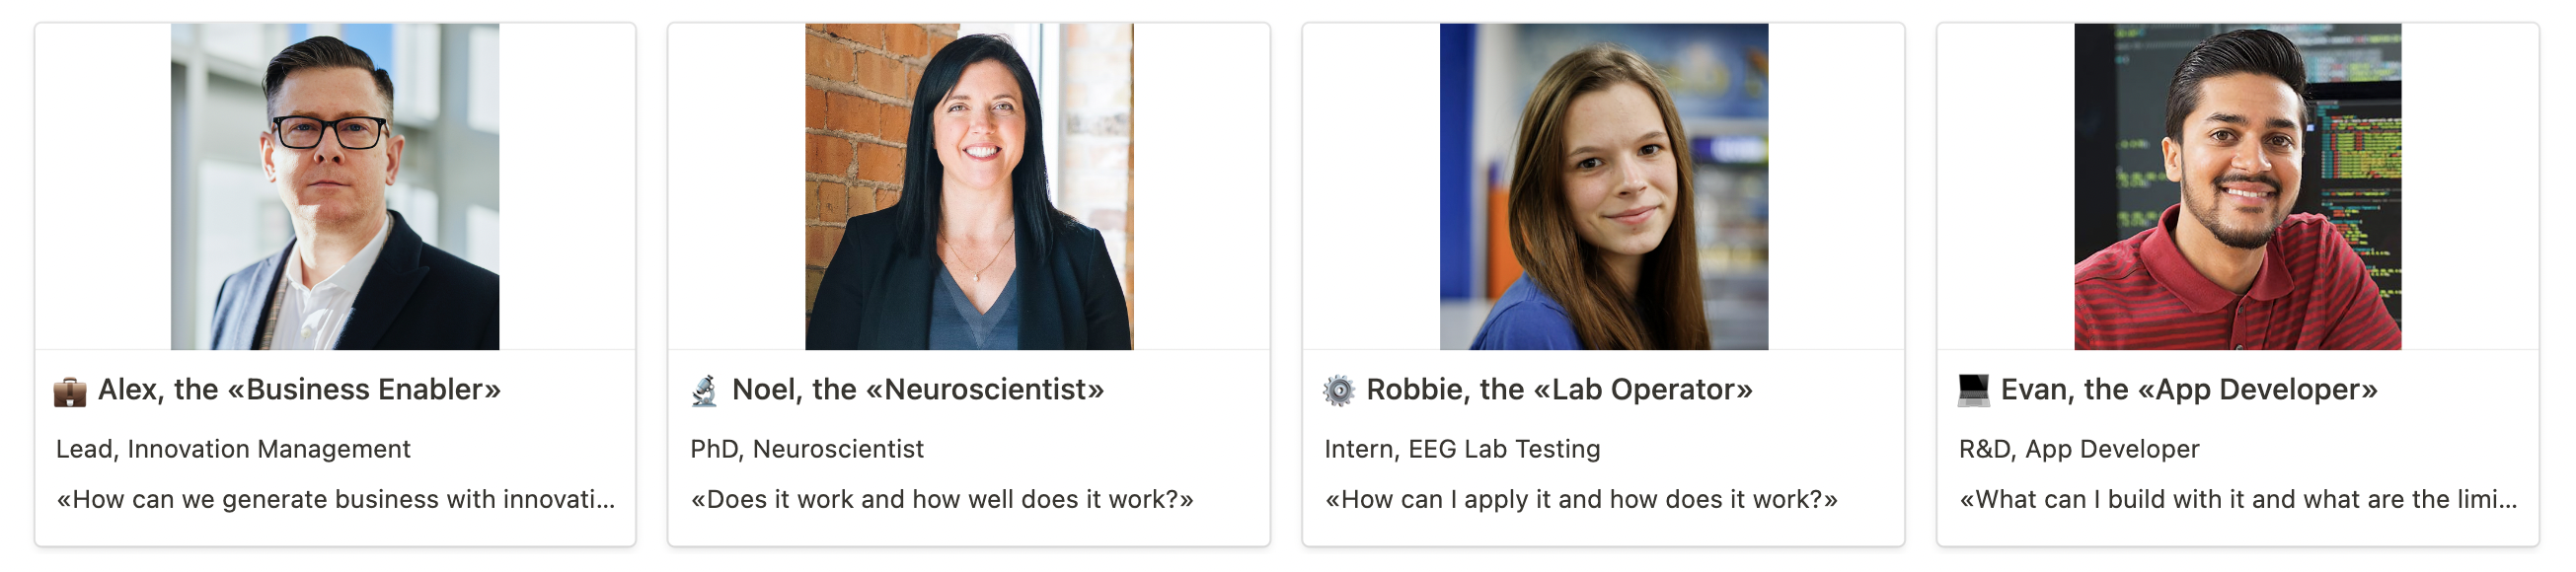
\includegraphics[width=\linewidth]{personas.png}
  \caption{IDUN's customer personas.}
  \label{fig:personas}
\end{figure}

Real people were then chosen to represent the personas as accurately as possible. The IDUN staff scoured their network to accomplish this. Finally, the author compiled a list of twenty individuals. Seven people were chosen from this list by the product manager and author and invited for an interview. The interview process was also planned in collaboration with IDUN's product manager and an industry UX expert, Laura Bendixen, who works as a UX designer at Blick.ch. The author completed the draft user interviews based on Laura's findings, which can be found in \autoref{appendix1-user-interviews}. All user interviews were conducted remotely and lasted no more than 1.5 hours. During the interviews, insights were jotted down on post-its. People working with BCIs or EEG were interviewed, as were PhD students, developers who had never worked with BCIs, and business-enablers from companies responsible for BCI-based accessibility.

The questions were non-leading open-ended, with the main goal of allowing interviewees to express themselves and capturing their perceptions of the BCI industry and upfront introduced IDUN vision and mission. The goal was to determine what software offerings a mass-market BCI-software device would need to provide, such as convincing developers who have never worked with BCI to include neuro-enhanced features, or convincing researchers to use IDUN's NIP in their research. The questions and answers were all about different things. More technically oriented people inquired about speed, performance, and privacy concerns (ergo more production-readiness thinking), whereas researchers inquired about signal quality, the ability to synchronise with other data streams, and access to raw data (more general applicability thinking). After the last user-interview, all post-its were compiled, similar insights were grouped and the product manager as well as the author categorised the most important insights into a list:

\begin{itemize}
  \item There are two main use cases: use the NIP for research purposes or build an app that goes intro production. These are two very important distinctions. Researchers would use the NIP to find out things about the brain in ways that were not possible before such as in easy remote experiment or real-life longitudinal experiments in non-lab environments. There the NIP is also in production per se, but not e.g. looking at possibly thousands or millions of users in a end-user facing app since the company or developer using the NIP would e.g. in the research use case have physical access to the hardware, since they would probably buy one or more devices and have them in their hands vs. when companies aiming at production-use cases would send the devices via their stores as white-labelled hardware and ergo not having actual physical access to each one's device. Maybe we can go even one further and say that if IDUN's device is so well distributed, that developers do not even need to sell the device on their own but just can assume that users have such earphones and then access the API. These three levels are very important for the architecture and design of the NIP and e.g. its GUI.
  \item Visual demos that are easily accessible for someone owning the hardware are important for all personas, most importantly an Alex. A visual and simple demo should demonstrate what one can do with the NIP from IDUN and inspire others to conduct research, build apps or enable business and opportunities. These demos need to explain to the different personas the different benefits, next to that also end-user should be able to try out the demos to see the benefits of BCI-enhanced technologies. People such as Evan should be able to adapt demos with their own codes to e.g. create their own version of e.g. a mind controlled game.
  \item The entire NIP needs to have as low-level control over the data flow, classification as possible but also with an option for less technical users to use it and build things, similar to e.g. AWS: AWS itself is only an API to use cloud IT resources, but they also have the AWS Console app to build everything via a GUI instead only via the API. What is very important here is that people such as e.g. Noels need to know exactly what for algorithms were used or what the methodologies for certain classifiers are in order to justify them and integrate them into their research. They do not actually need raw data access as plotting functionality would also be enough, therefore IDUN's NIP should have somewhere functionalities to plot and visualise data.
  \item In order to ease the use of the GUI and the API of the NIP, IDUN needs to provide, next to a satisfying documentation, libraries for certain environments that make the unobtrusive implementation of the NIP easier. Such as e.g. providing a client-side JavaScript package that is lean and easy to use that can be integrated simply into existing apps. Examples for such code integration would also need to be provided by IDUN so that people like Evan can easily adjust them and more quickly start integrating them into their apps or research codebases. The personas would need to be able to abstract the brand IDUN as much as possible away as e.g. Intel is doing with their Intel-inside ingredient strategy \citep{intel_ingredient_nodate}.
  \item End-users need control over their data so that other companies accessing the NIP API cannot collect the data on their servers and and do everything what they want with it. Imagine if e.g. the operating system layer of ones smartphone would not offer an opt-in mechanism for the cameras, then 3rd-party developers could just install spyware and record without the user giving permission for it. When e.g. users start to use multiple apps with an NIP integration, there needs to be some way to control the opt-in and data access without the app developers having any saying on the decisions. There needs to be a technical limitation from the side of the hardware or the cloud to ensure user privacy and data security for end-users.
  \item Researchers are very interested in the raw EEG data and the synchronisation possibilities with certain protocols such as LSL to combine e.g. a heart rate sensor with the EEG collected from IDUN's hardware. The NIP software offering need to give enough freedom to combine the data without letting researchers send all the other collected data sent to IDUN but with also still respecting the privacy of users.
\end{itemize}

These insights were key to find out that there needs to be enough freedom to do research on raw data, but without giving out raw data in production to protect end-user's privacy. Therefore some opt-in mechanism must take place. Also, there needs to be an SDK that can be implemented into end-user facing applications that directly connects to the hardware without the need to download a companion app from IDUN itself.

\subsection{Invention of N/CI}
\label{chapter4-invention-of-nci}
% make the connection why the author talked about it in the beginning already

\subsection{Web-first approach}
\label{chapter4-web-first-approach}
% mention dog feeding and Vercel

\subsection{Python to WebAssembly}
\label{chapter4-python-to-webassembly}
% mention sprint that we committed to that one
% sushi principle

\subsection{Kubernetes and Fargate}
\label{chapter4-kubernetes-and-aws-fargate}
% quickly explain why microservices
% mention workshop with nuvibit (expert interview)
% mention conversation with Jules (expert interview)
% mention centralised system rather than distributed

\subsection{Kafka and Kinesis}
\label{chapter4-kafka-aws-kinesis}
% mention workshop with nuvibit (expert interview)

\subsection{IaC with Terraform}
\label{chapter4-iac-with-terraform}
% mention workshop with nuvibit (expert interview)
% mention workshop with sascha from piavita

\subsection{MQTT and WebSocket}
\label{chapter4-mqtt-and-websocket}
% show image of andy on the whiteboard
% talk about compression and data structure of the EEG data

\subsection{Python SDK}
\label{chapter4-python-sdk}
% mention internal discussions with Michel (group discussion)
% mention GitHub limitation of private PyPI and registry in general
% mention again the no focus on GUI part from before

\section{Key aspects}
\label{chapter4-key-aspects}

\subsection{Stream-based events}
\label{chapter4-stream-based-events}
% explain event based architecture and the paradigm-shift in building stream based architectures
% talk about concurrency

\subsection{Critical and non-critical}
\label{chapter4-critical-and-non-critical}
% mention the concept from the book and batch processing

\subsection{Hardware-accelerated encryption}
\label{chapter4-hardware-accelerated-encryption}
% mention server-side rendering for privacy
% mention discussion with Andy

\subsection{Per-device auth and opt-in}
\label{chapter4-user-side-opt-in}
% show opt-in wireframes

\subsection{Graph database}
\label{chapter4-graph-database}

\subsection{Feature store and MLOps}
\label{chapter4-feature-store-and-mlops}
% explain MLOps and outlook with Kubeflow
% mention data lakes and data warehouse
% mention internal SDK for feature extraction and experiments
% what is feature extraction and the process
% show image from Wadda

    % However, in practice, it appears that simply making data available quickly—even if it is in a quirky, difficult-to-use, raw format—is often more valuable than trying to decide on the ideal data model up front [54].
